\documentclass{article}
\usepackage{graphics}
\usepackage{indentfirst}
\usepackage{amsmath}
\usepackage{algorithm}
\usepackage{algorithmic}
\usepackage{bm}
\usepackage{setspace}
\usepackage{graphicx}
\usepackage{float}
\author{Ruichen Wang}
\title{Ad Click Prediction}
\begin{document}
\maketitle
\begin{abstract}
There are a lot of algorithms designed for ad ctr prediction. Those algorithms take contextual and historical features as inputs, often combines massive feature engineering work, then predict whether or not the user will click some certain ads. Here I'd like to summarize some popular traditional solutions and recent deep learing technics.
\end{abstract}

\tableofcontents
\section{Online Advertising and Linear Model Sparsity}
For learning in massive scale, generalized linear models have many advantages.  Easily implement, memory saving, efficient training on streaming data.

Supposing we choose logistic regression as our model. Given feature $x_{t} \in R^{d}$, model parameter $w_{t}$. we can predict $p_{t}=\sigma (w_{t} \cdot  x_{t})$, where $\sigma(x)=\frac{1}{1+exp(-x)}$ is the sigmoid function. And our observation $y_{t} \in \{0,1\}$. The log loss can be easily denoted as :
$$\mathcal{L}(w_{t})=-y_{t}log p_{t}-(1-y_{t})log(1-p_{t})$$
It is obvious that:
$$\frac{\partial \mathcal{L}}{\partial w}= (\sigma(w \cdot x_{t})-y_{t}) x_{t} = (p_{t}-y_{t})x_{t}$$
And this gradient is all we need for optimization purpose. 
\subsection{Online Gradient Descent (OGD)}
OGD is essentially the same with SGD. OGD can provide excellent prediction accuracy with minimum computing resources. However, as $x$ might have billions of dimensions, the size of the final model is another key consideration. Here we want the $w$ be sparse, while keep the accuracy or little accuracy loss.

However, OGD is not good at producing sparse result. In fact, simply adding subgradient penalty will never induce sparsity.
\subsection{Truncated Gradient (TG)}
There is a very simple solution to produce sparse solution. Just rounding small weights to 0. but doing so may cause some problems, because a weight may be useless or small because it has been updated only once, or at the begining of the training. 
Truncated gradient\cite{DBLP:journals/jmlr/DuchiHS11,DBLP:journals/jmlr/LangfordLZ09} introduce another natural method to round small coefficients.

\begin{figure}[h]
\centering
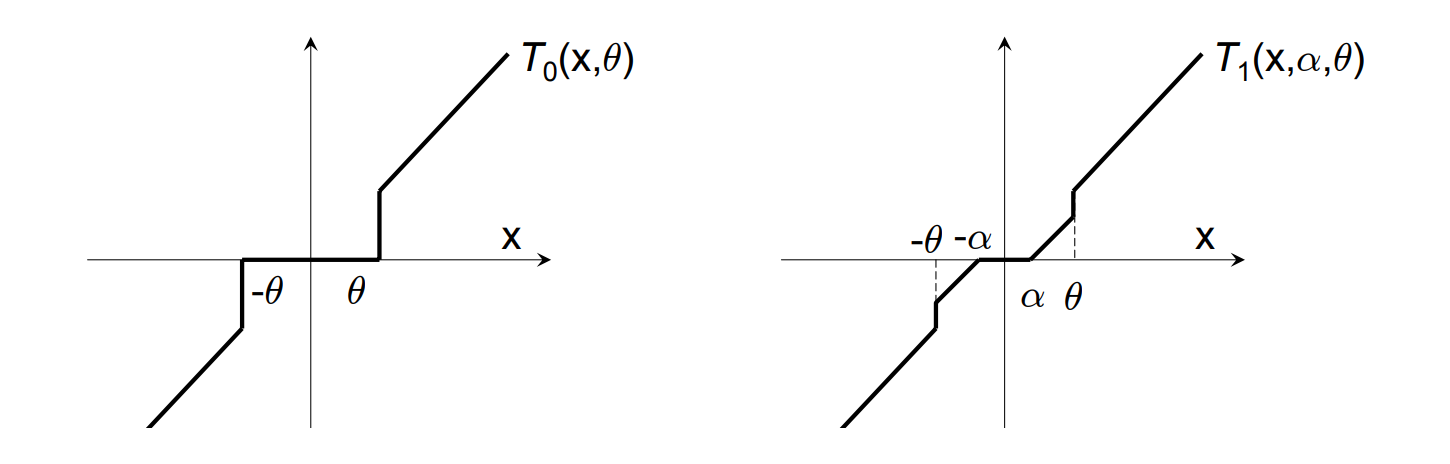
\includegraphics[width=4in,height=1.3in]{figure1}
\caption{Plots for the truncation functions below.}
\end{figure}

\noindent
For each K steps, perform simple coefficient rounding.
$$ T_{0}(v_{j},\theta)=\left\{
\begin{array}{lcl}
0       &      & {if \  \left| v_{j} \right| \leq \theta}\\
v_{j}     &      & {otherwise}
\end{array} \right. $$
For each K steps, truncate gradient.
$$ T_{1}(v_{j},\alpha,\theta)=\left\{  
\begin{array}{lcl}
max(0,v_{j}-\alpha)       &      & {if \ v_{j} \in [0,\theta]} \\
min(0,v_{j}+\alpha)       &      & {if \ v_{j} \in [-\theta,0]} \\
v_{j}     &      & {otherwise}
\end{array} \right. $$
\subsection{Forward-Backward Splitting (FOBOS)}
In FOBOS\cite{DBLP:journals/jmlr/DuchiS09}, the problem is considered as two parts,
$$f(w)+r(w)$$
where $f$ is the empirical loss and $r$ is a regularization term that penalized for excessively complex vectors.
FOBOS updates the $w$ in 2 steps, forward-looking subgradients and forward-backward spliting. May sound complex, Actually it's very simple. 
$$w_{t+\frac{1}{2}}=w_{t}-\eta_{t} g_{t}$$
$$w_{t+1}=\mathop{\arg\min}_{w_{t}} \left \{ {\frac{1}{2} || w_{t}-w_{t+\frac{1}{2}}||}^{2}+\eta_{t+\frac{1}{2}}r(w_{t}) \right \} $$
The first step is apply the gradient to the weight. The second step mainly contributes to the sparsity.It can be viewed as (\textrm{i})let the updated weight be close to the previous one (\textrm{ii}) attain a low complexity.
\subsection{Regularized Dual Averaging Algorithm (RDA)}
RDA\cite{DBLP:journals/jmlr/Xiao10} condsider the learning variables are adjusted by solving a simple minimization problem that involves the running average of all past subgradients of the loss function and
the whole regularization term, not just its subgradient.
$$w_{t+1}=\mathop{\arg\min}_{w} \{\frac{1}{t}\sum_{i=1}^{t}\langle g_{i},w\rangle +\Psi(w)+\frac{\beta_{t}}{t}h(w)  \}$$
At each iteration, this method minimizes the sum of three items: (\textrm{i}) all previous subgradients (dual average). (\textrm{ii})the original regularization funciton ($\lambda ||w||_{1}$). (\textrm{iii}) an additional strongly convex regularization term($\frac{1}{2}||w||^{2}_{2}$). It can be denoted as :
$$w_{t+1}=\mathop{\arg\min}_{w} \{\frac{1}{t}\sum_{i=1}^{t}\langle g_{i},w\rangle +\lambda ||w||_{1}+\frac{1}{2}||w-0||^{2}_{2}  \}$$

In result, RDA producs even better accuracy vs sparsity tradeoffs than FOBOS. 

\subsection{Follow the Proximally Regularized Leader (FTRL-Proximal)}
FTRL \cite{DBLP:journals/corr/abs-1009-3240} is a hybrid of FOBOS and RDA, and  significantly outperforms both on large real-world dataset.
$$w_{t+1}=\mathop{\arg\min}_{w} \{ g_{1:t} \cdot w+t\lambda ||w||_{1} +\frac{1}{2} \sum_{s=1}^{t}\sigma_{s} || w-w_{s}||^{2} \}$$
where $\sigma$ is the learning rate schedule, such that $\sigma_{1:t}=\frac{1}{\eta_{t}}$.
The update of this fomula is actually very simple. As the fomula above can also be written as :
$$(g_{1:t}-\sum_{s=1}^{t}\sigma_{s}w_{s}) \cdot w 
+\frac{1}{\eta_{t}}||w||_{2}^{2}
+\lambda_{1}||w||_{1}
+const$$
If we store $z_{t-1}=g_{1:t-1}-\sum_{s=1}^{t-1}\sigma_{s}w_{s}$ in memory. At each round t, we update $z_{t}$:
$$z_{t}=z_{t-1}+g_{t}+(\frac{1}{\eta_{t}}-\frac{1}{\eta_{t-1}})w_{t}$$
and the $w_{t+1}$ can be solved in closed form on: 
$$w_{t+1}=\left\{  
\begin{array}{lcl}
0 & & {if \ |z_{t}|\leq \lambda_{1} } \\
-\eta_{t}(z_{t}-sgn(z_{t})\lambda_{1}) & & {otherwise} \\
\end{array} \right. $$
Thus FTRL-Proximal stores $z$ in memory, whereas OGD stores $w$. 
\paragraph{Per-coordinate leaning} Standard online learning gradient descent suggest using a global learning rate schedule $\eta=\frac{1}{\sqrt{t}}$, which is common for all coordinates. As some coordinate updates frequently and some not. It makes more sense to represent the gradient per coordinate:
$$\eta_{t,i}=\frac{\alpha}{\beta+\sqrt{\sum_{s=1}^{t}g^{2}_{s,i}}}$$
$\beta$ is simply for numeric stable sake, ensures that early learning rate not too high. $\beta=1$ is usually good enough. 
\section{Collaborative Filtering}
\subsection{Factorization Machines (FM)}
In recommender system, we may want the model to be able to estimate interactions between large feature dimensions, while keeping the sparsity.
FM \cite{DBLP:conf/icdm/Rendle10} is designed to deal with highly sparse features.It has linear complexity, and can work with any real valued feature vector. It can be used in many prediction task like regression, binary classification and ranking. 
\begin{figure}[H]
\centering
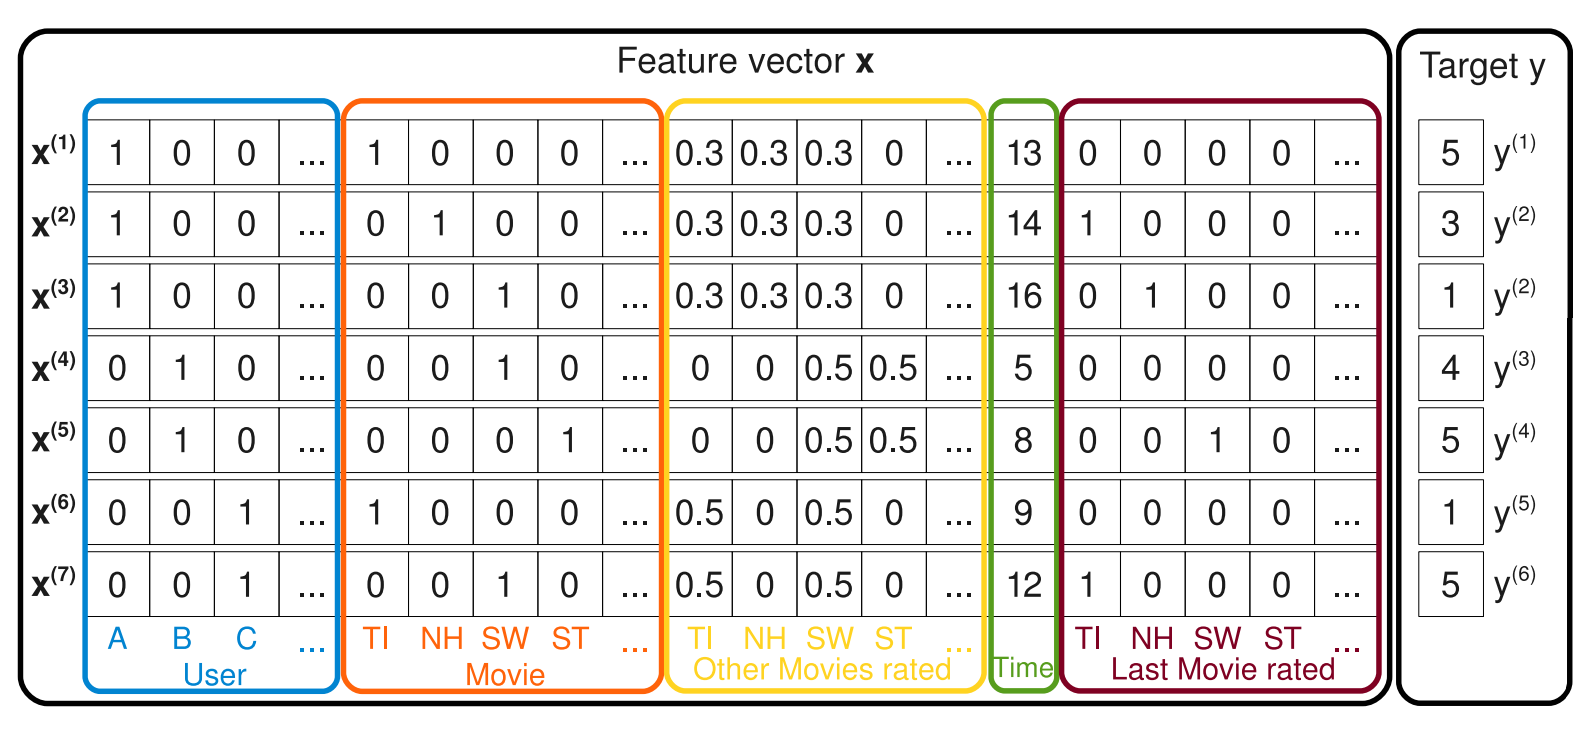
\includegraphics[width=5in,height=2in]{figure2}
\caption{Sparse user features and target y.}
\end{figure}
\paragraph{Model equation} Given $x \in R^{n}$, the model parameters that have to be estimated are $ w_{0} \in R, \textbf{w} \in R^{n}, \textbf{V} \in R^{n \times k}$.
$$\widehat{y}= w_{0}+\sum_{i=1}^{n}w_{i}x_{i}+\sum_{i=1}^{n}\sum_{j=i+1}^{n}\langle \textbf{v}_{i} ,\textbf{v}_{j} \rangle x_{i}x_{j}$$
where 
$$\langle \textbf{v}_{i} ,\textbf{v}_{j} \rangle =\sum_{m=1}^{k}v_{i,m} \cdot v_{j,m}$$
Based on the theory that for any positive definite matrix (semi-positive definite) \textbf{w}, there exists a matrix \textbf{v} such that $\textbf{w}=\textbf{v} \cdot \textbf{v}^\mathrm{T}$ if k is not limited. In practice, we often pick a small $k$ for better generalization
and thus improved interaction matrices under sparsity.
\paragraph{Computation}
If we follow the straight forward computation, the cost will be $O(kn^{2})$. We can apply some mathematics transformations to reduce the computation to linear time $O(kn)$.
\begin{align*}
\sum_{i=1}^{n}\sum_{j=i+1}^{n}\langle \textbf{v}_{i} ,\textbf{v}_{j} \rangle x_{i}x_{j}
&= \frac{1}{2} \sum_{i=1}^{n}\sum_{j=1}^{n}\langle \textbf{v}_{i} ,\textbf{v}_{j} \rangle x_{i}x_{j} -\frac{1}{2}\sum_{i=1}^{n}\langle \textbf{v}_{i} ,\textbf{v}_{i} \rangle x_{i}x_{i} \\
&= \frac{1}{2}\sum_{m=1}^{k}\left( \left(\sum_{i=1}^{n}v_{i,m}x_{i}\right)^{2} -\sum_{i=1}^{n}v_{i,m}^{2}x_{i}^{2} \right)
\end{align*}



\subsubsection{ALS}
\subsection{FFM}
\section{Incorporate with Deep Learing}
\subsection{FNN}
\subsection{PNN}
\subsection{Deep and Wide}
\subsection{DeepFM}
\subsection{DNN}

\bibliographystyle{plain}
\bibliography{ref}

\end{document}

























